\chapter{Operations \& Logistics}
\setlength{\parindent}{15pt}
\label{ch:oper_logi}

\section{Operations \& Logistics Concept Description}
\label{sec:oper_logi_conc_desc}

\begin{figure}[htb]
    \centering
    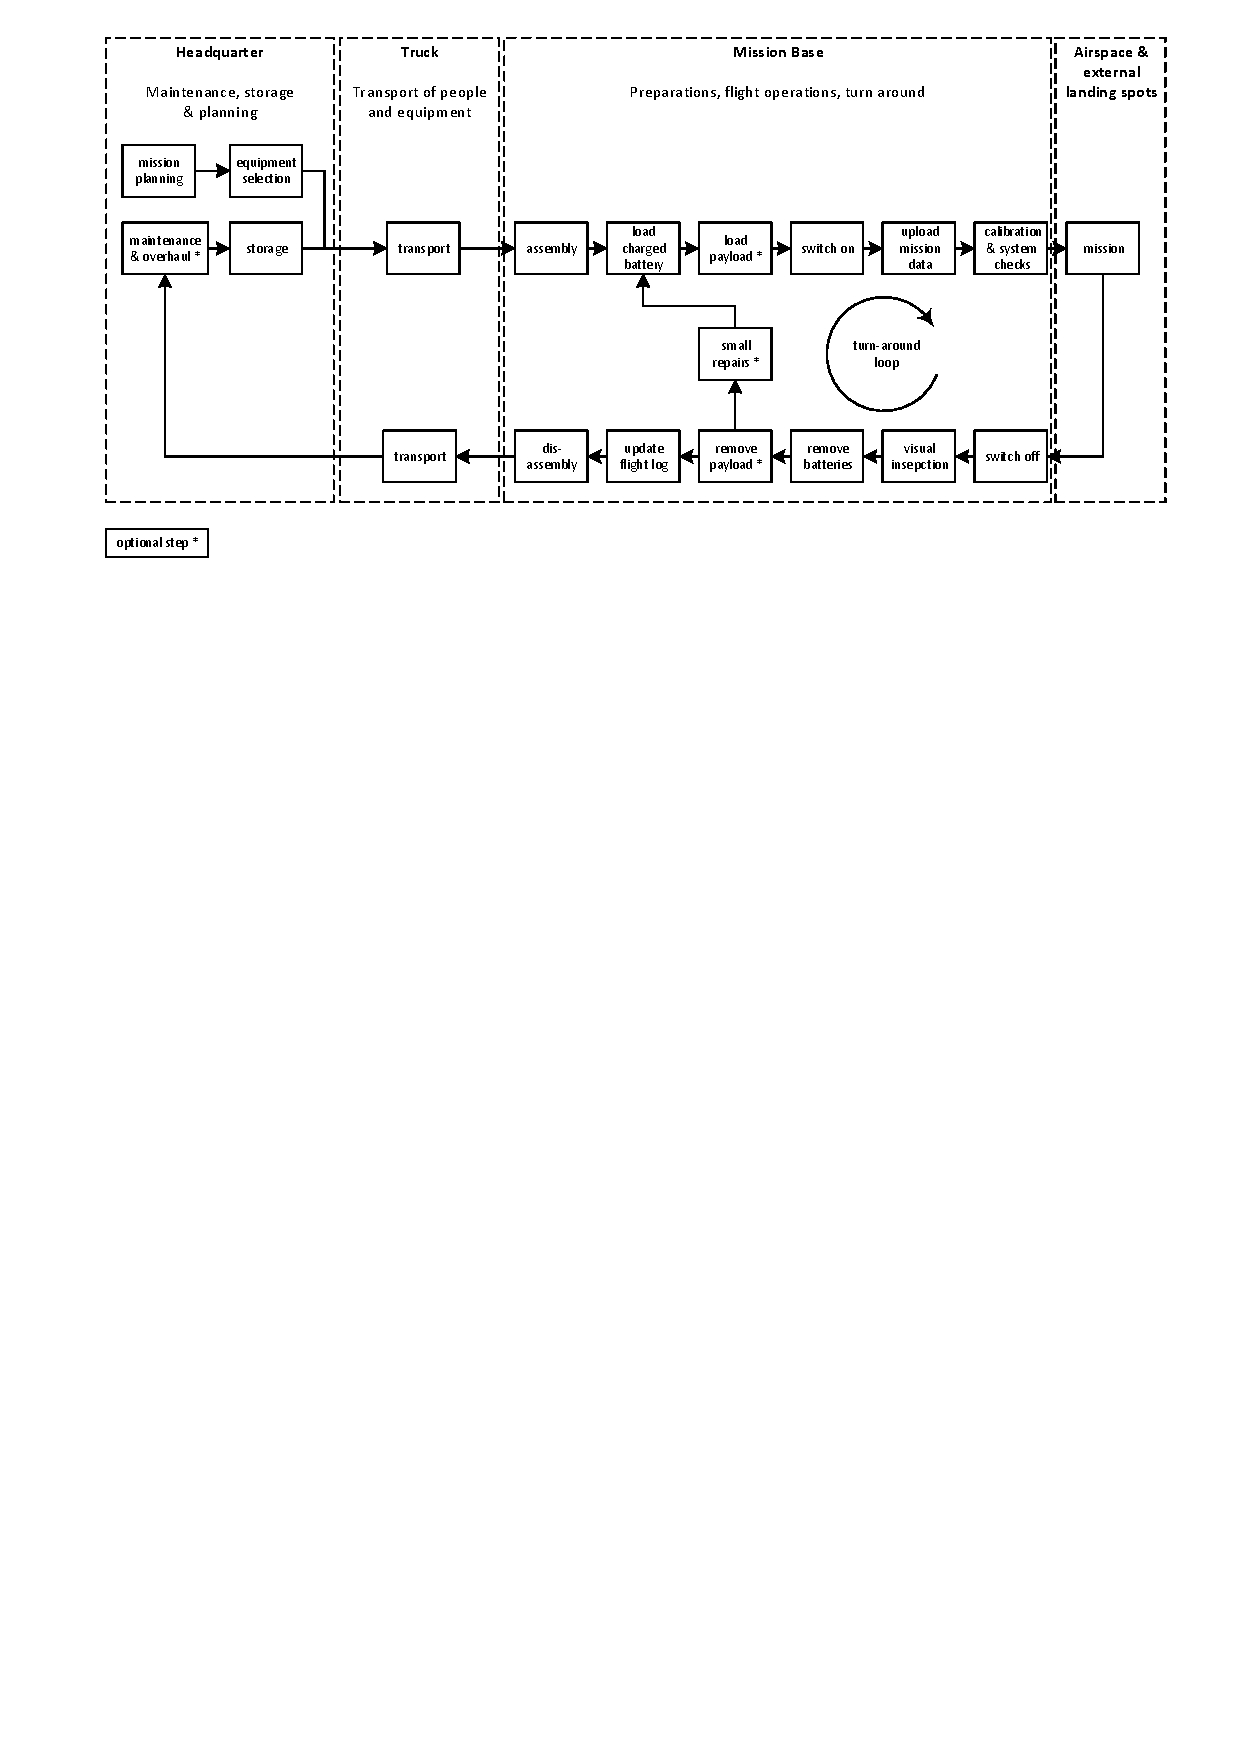
\includegraphics[width=1\textwidth]{OperationsLogistics/Figures/operations_logistics.pdf}
    \caption{Operations \& Logistics Flow Diagram}
    \label{fig:opslogsdig}
\end{figure}

\autoref{fig:opslogsdig} shows the the operations and logistics flow diagram for what this group expects to be typical operating conditions. It is assumed that the UAV operator has a main facility, from which the UAV, staff and mission relevant equipment are transported to a mission base at which flight operations take place. Naturally, variations to this scheme are possible, e.g. a parcel company may exclusively operate from its main facility, or long-range missions require a turn-around at a remote location, but for the sake of brevity only the most general case is presented.
The starting and end point of each mission is the so-called headquarters, the place where maintenance and storage takes place. Based on customer input a mission plan is set up, which determines the kind of resources that are required. Next to one or more UAVs, this includes staff on site, equipment such as the ground station, spare parts, additional batteries and a transport vehicle. Once the preparation is done, everything is loaded into a vehicle and transported to the location where the UAV is intended to take off and land. \autoref{fig:transport} shows the UAV body in disassembled state within a standard size van, where the remaining space can be filled with support equipment.
Once on site, the equipment needs to be unloaded and the UAV assembled into its operational form. A charged battery is then loaded, followed by the payload, which can also consist of another set of batteries. The system is switched on, the mission relevant data is uploaded to the on-board computer and an automated instrument calibration and readiness check performed. The UAV is now ready to fly and carry out its mission. After its return, the system is switched off for safety reasons, visually inspected and stripped off its batteries. The next steps depend on the kind of mission in question. If another flight is scheduled, the payload can be replaced and minor repairs taken out, e.g. replacing a damaged propeller blade. Once the battery is recharged or replaced by a full one, a new flight cycle can start. In case the mission does not comprise a turn-around or substantial damage was detected, the digital flight log is updated and the UAV disassembled. After loading all equipment the transport back to the headquarter takes place, where scheduled maintenance and all levels of repairs are carried out. Once the work is documented and approved, the equipment is stored and ready for the next mission.

\begin{figure}[htb]
    \centering
    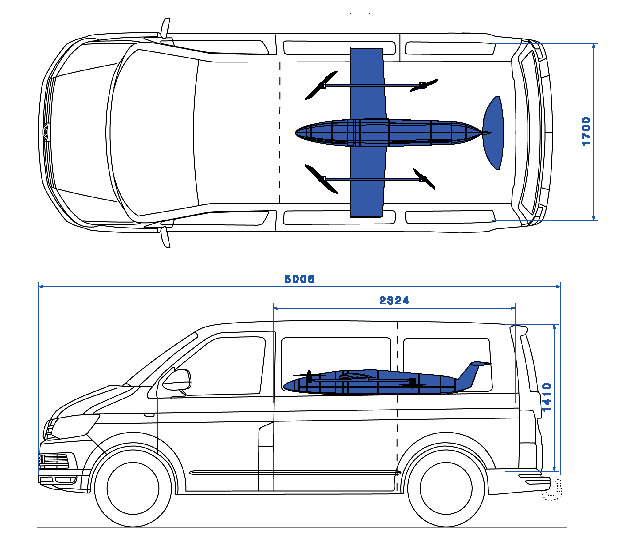
\includegraphics[width=0.7\textwidth]{OperationsLogistics/Figures/storage.pdf}
    \caption{UAV Van Transport}
    \label{fig:transport}
\end{figure}



\section{RAMS Characteristics} %chris somebody may write about maintainability if bored
\label{sec:rams_char}

In this section, the reliability, availability, maintainability and safety (RAMS) characteristics are presented. First, different safety critical functions are presented together with procedures to be carried out in their respective case. These procedures might include making use of a redundant system or emergency procedures to be carried out. The section concludes with a list of different maintenance activities. 
\nomenclature[A]{RAMS}{Reliability, Availability, Maintainability and Safety}

\subsection{Reliability and availability}

As explained in \autoref{ch:avio_grou_hand}, the UAV is highly dependant on the autopilot. Only for control in close range manual control is possible and even then the reliability of the flight controller, in order to manage the data flow, is of major importance. For this reason, the most critical functions are the ones needed for autonomous flight. The following paragraphs will explain one by one the failure of the different UAV components.

First, the flight controller bases all of its decision on the data it receives by the sensors. Wrongly assumed attitude or airspeed result in wrong actions and might in worst case lead to crashes. In order to prevent this from happening, redundancy is provided for the critical sensors. At least two accelerometers, barometers, magnetometer, gyroscopes and airspeed sensors are used in order to calculate attitude. The probability that all of them fail during a single mission can be assumed negligible. In case of object avoidance or ground distance sensor failure, the UAV will still be able to perform its mission, however the probability of crashing into an obstacle increases significantly and thus an emergency landing is performed. GPS data, with the help of pressure sensors will be used in order to determine a ground distance estimate during landing. GPS failure will result in the inability to determine the position and hence in mission failure. In this case also an emergency landing will be performed and a notification including last known position and failure reason will be send to the ground station. 

Another flight controller failure comes from the power source. Battery failure includes an empty battery, burnout or overvoltage. Empty battery will result in total failure, burnout and overvoltage can result in damaged hardware. In order to prevent this, the flight controller uses a power brick to manage the power supply. It sends useful information as battery status and battery level to the flight controller. This reduces the chances of wrong voltage distribution and makes it possible for the flight controller to perform a return to base procedure in case the energy level drops below a certain threshold. Regular inspection and replacement of the battery will also reduce the probability of battery failure. 

Then, servos are used throughout the system for either engine tilting mechanisms or control surface deflection. In the former, either one or more engines are stuck in horizontal or vertical position. In case only one or two engines are stuck, the remaining ones can be used to fly the drone to a safe location and perform a landing. If stuck in horizontal mode however, a safe vertical landing will not be possible anymore and a horizontal landing has to be performed. The impact of tilting actuator failure is minimal, as horizontal flight is still possible using only one engine. If actuators are stuck in vertical mode, a safe vertical landing can be performed. A more critical case is failure of a control surface. Aileron failure results in an inability to perform rolling action. This can be counteracted by the rudder and slight tilting of the engines. Rudder failure is counteracted using different thrust at each side and elevator failure is compensated for by tilting the front or back engines. Although redundancy is provided for control surface failure, a return to base procedure will be carried out in such a case to diminish the risk of further damage. 

After that, engine failure is a critical risk that has to be considered. One engine failure can be compensated by the rudder in horizontal flight, however vertical flight will not be possible anymore. In this case, also the forward propellers are used in order to generate enough thrust to perform a return to base procedure. Then in case of more engine failures, horizontal flight will be performed using the remaining engines and depending on the distance towards the base a new landing location might have to be chosen. In case the engines fail during vertical flight, no other option but to perform a emergency landing. This will not be possible in all cases but the flight controller will try to minimise the landing impact. 

The last failure to be considered is the failure of the telemetry link and the RC link. In this former case, no more waypoints can be send to the drone and the drone can not send updates regarding its flight conditions. If both links become unavailable, the drone will perform a return to base action resulting in mission failure. In order to minimise the risk of telemetry failure, missions always have to be planned and configured before UAV take-off. This makes it possible for the drone to perform its initial planned mission in case something goes wrong with the return procedure during link failure. 

In conclusion, all the critical systems used in the UAV system either have redundancy in case of failure or a safe procedure that can be performed limiting the damage. The most critical failure is an engine failure during vertical flight. Here no other option can be performed but landing the drone vertically while trying to minimise the impact. The reliability of the chosen engines however is high as explained in \autoref{ch:powe_prop}. As on top of that, the drone spends most of its mission time in horizontal flight, the probability of this event to occur is minimal. The modular design of the UAV ensures the availability of the drone, as in case of a failure, only the specific parts have to be exchanged. This can be performed without major complications. 

\subsection{Maintenance}

Next to the reliability aspect, availability and safety aspects strongly depend on the necessary maintenance procedures for the UAV. Extra maintenance will results in better safety aspects however, the availability will decrease. In case no maintenance is performed, the safety of the UAV can not be ensured anymore and if there is an unexpected failure the UAV will be unavailable for a longer period. The following shows different maintainability procedures depending on how often they have to be carried out. 
\newline


\paragraph{Start of mission}     \begin{enumerate}
    \item Check previous error log for previous mission problems and ensure that they have been fixed. 
    \item Make sure that battery is disconnected. 
    \item Assemble wing to fuselage.
    \item Inspect all connectors, propeller blades and wings for cracks. If cracks are present they have to be reported and maintenance might be necessary depending on the crack length and thickness. 
    \item Mount payload and connect a full battery.
    \item Establish cellular connection from UAV to ground station.
    \item Configure all waypoints needed for mission. 
    \item Control correct functioning of servos and engines using RC link. If an error occurs in the functioning it has to be reported and the mission will be aborted.
    \item Check correct calibration of sensors.
\end{enumerate}

\paragraph{End of mission} 
\begin{enumerate}
    \item Check internal error log for probable errors. If errors are present report them. 
    \item Disconnect battery and connect it to charger.
    \item Quick inspection on damages that might have occurred during mission.
    \item Disassemble wing from fuselage and clean different parts.
\end{enumerate}

\paragraph{Monthly Basis}
\begin{enumerate}
    \item Check all internal software for system updates and update them if necessary. 
    \item Full external inspection for cracks.
    \item Recalibration of all sensors.
\end{enumerate}






















